%\documentclass[10pt]{beamer}
%\usetheme{amcg}
%\usepackage{subfigure}

%\begin{document}

\section{Advection of a top hat}

\begin{frame}
  \frametitle{The top hat}
  \begin{itemize}
  \item Top hat distribution of a tracer, advected with prescribed velocity.
  \item Simple, fast: ideal laboratory to experiment and play.
  \item Compare CG, CV, DG discretisations.
  \end{itemize}

  \begin{figure}
    \centering
    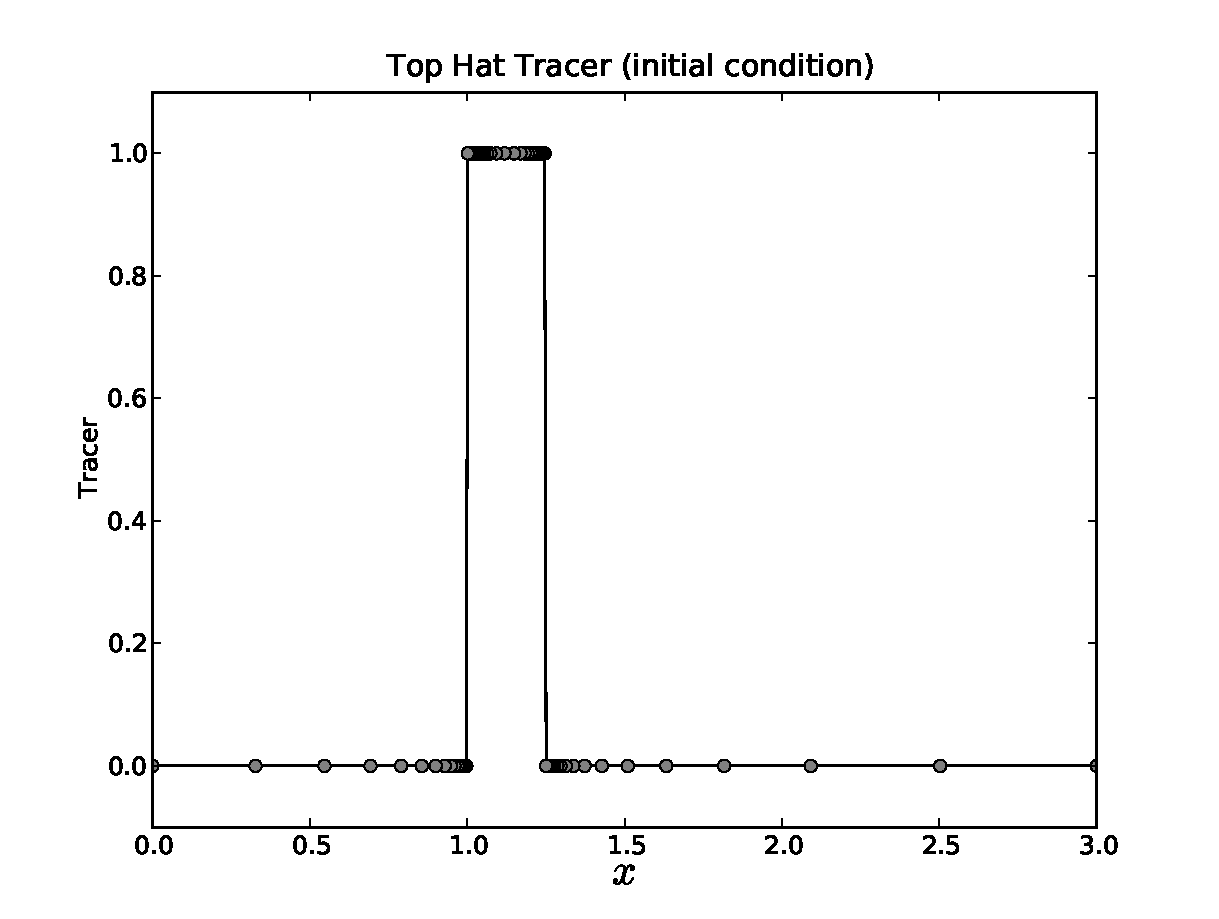
\includegraphics[width=0.45\textwidth]{./top_hat/top_hat_ic.pdf}
    \caption{Initial top hat distribution.}
  \end{figure}
\end{frame}

\begin{frame}
  \frametitle{The top hat}
  \begin{figure}[ht]
    \begin{tabular}{ccc}
      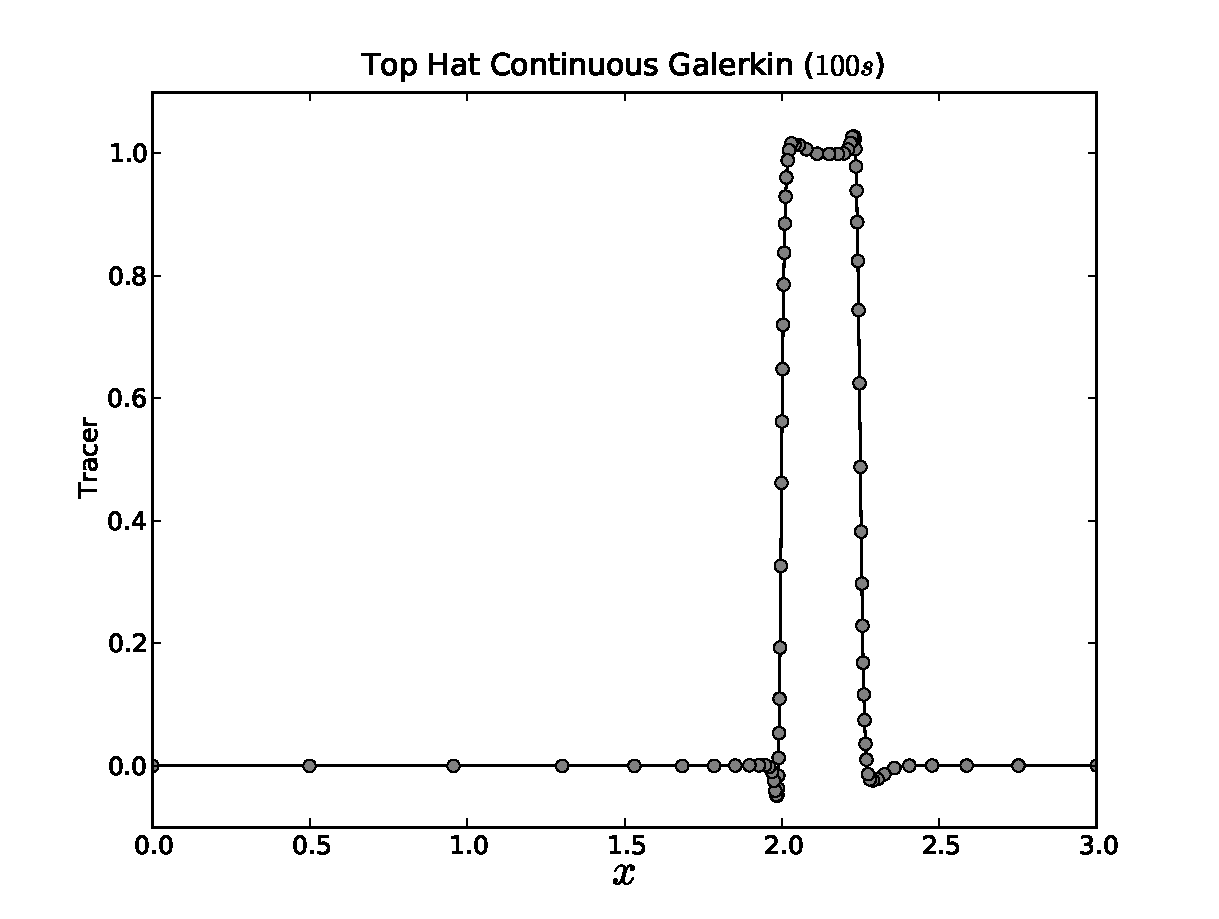
\includegraphics[width=3.5cm]{./top_hat/top_hat_cg.pdf} &
      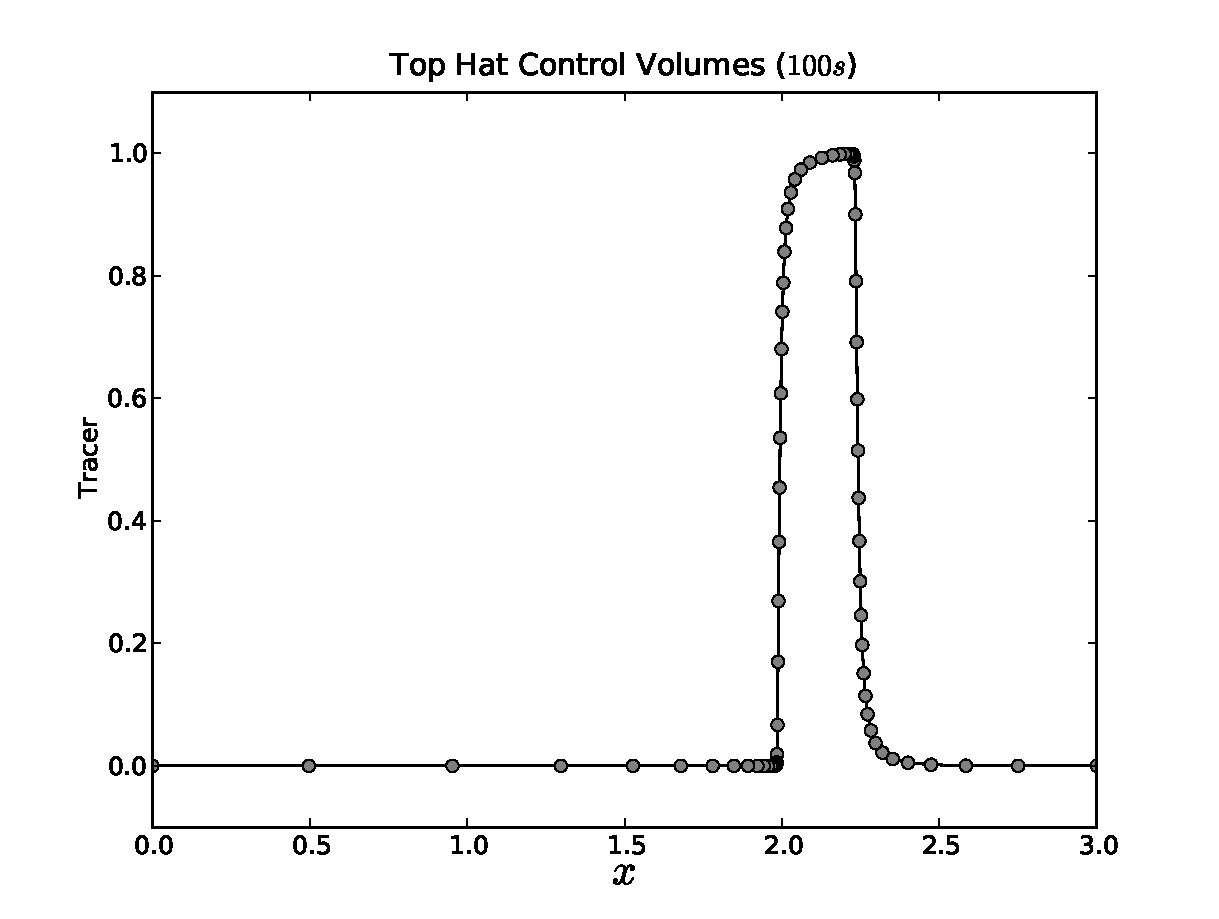
\includegraphics[width=3.5cm]{./top_hat/top_hat_cv.pdf} &
      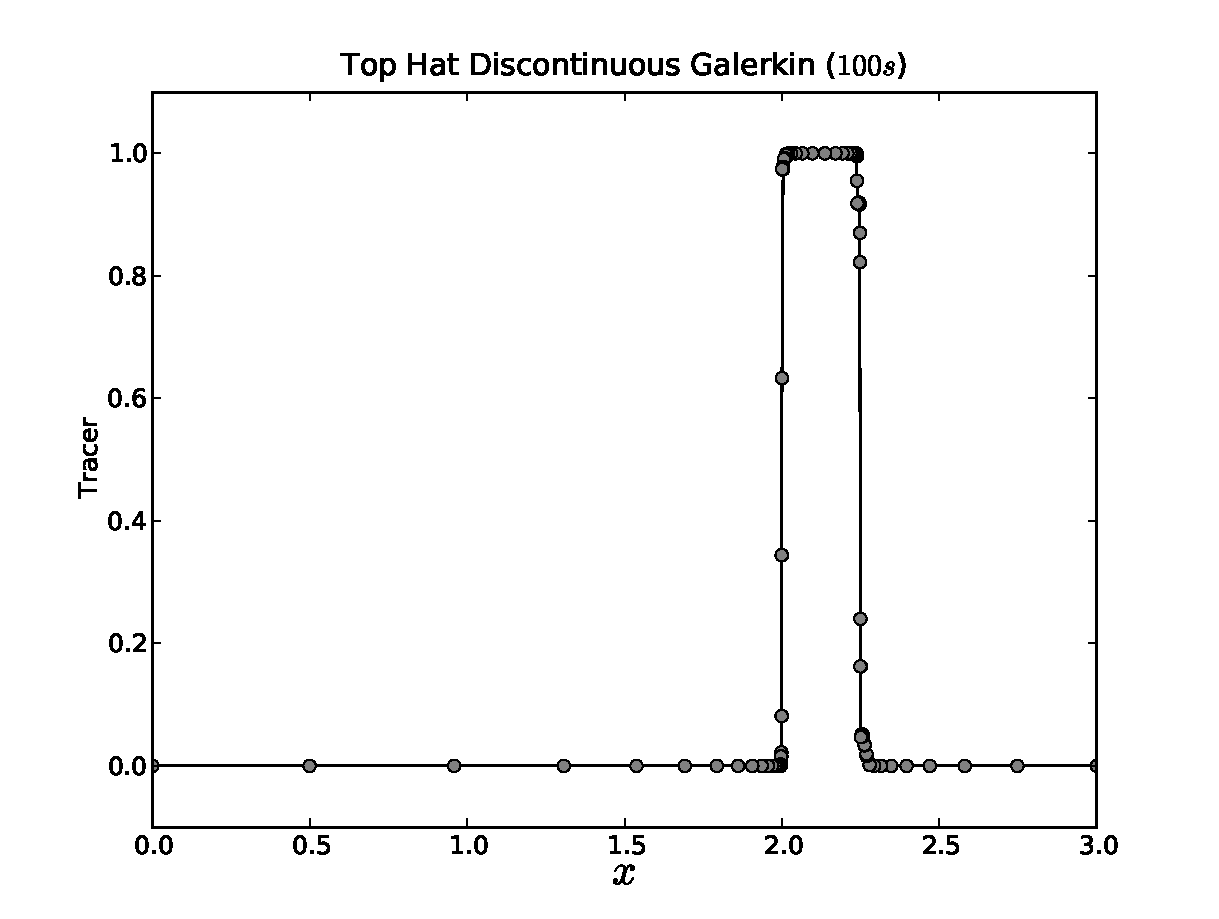
\includegraphics[width=3.5cm]{./top_hat/top_hat_dg.pdf} \\
      CG & CV & DG
    \end{tabular}
  \end{figure}
\end{frame}

\begin{frame}
{\small
  \begin{block}{Continuous Galerkin}
    \begin{itemize}
      \item Basic finite element discretisation
      \item Not good for advection of sharp discontinuities
      \item SUPG stabilisation applied in this case
    \end{itemize}
  \end{block}
  \begin{block}{Control Volume}
    \begin{itemize}
      \item Simple and efficient, sometimes diffusive
      \item Need to choose an interpolation method
      \item Here, ``FiniteElement'' interpolation with Sweby limiter used
    \end{itemize}
  \end{block}
  \begin{block}{Discontinuous Galerkin}
    \begin{itemize}
      \item Popular for advection problems
      \item Slope limiters still needed near discontinuities to prevent overshoots
    \end{itemize}
  \end{block}
}
\end{frame}

\begin{frame}
  \frametitle{Exercises}
  \begin{itemize}
    \item Turn off SUPG stabilisation for the CG case and see what it does.
    \item Change the resolution of the adapted meshes.
    \item Change the control volume interpolation method to HyperC.
  \end{itemize}
\end{frame}

%\end{document}
